\chapter{Methods}
\label{cha:Methods}

%As the bees have been showing a range of different types of trajectories, ranging from random seeming walks, over preferred movement in the vicinity of the walls and and almost straight uphill walks to no movement at all and often a mixture of those types a system to describe them all was developed. In molecular chemistry and molecular biology 

\begin{table}[H]
\caption{Description of the used variables in order of appearance}
    \centering
    \begin{tabular}{p{1.4cm}|p{12.4cm}}
         \textbf{Variable} & \textbf{Description} \\
         \hline
         \hline
         $m_{i}$ & inertial mass of a particle  \\
         \hline
         $\vec{x_{i}}$ & position of a particle   \\
         \hline
         $\gamma$ & friction coefficient  \\
         \hline
         $t$, $t'$ & time domain of the real time \\
         \hline
         $v_{0}$ & driving velocity of a particle/bee\\
         \hline
         $\hat{n}_{i}$ & orientation of a bee \\
         \hline
         $V$ & temperature gradient \\
         \hline
         $D$ & Diffusion coefficient \\
         \hline
         $\eta$ & Gaussian distributed white noise \\
         \hline
         $\delta$ & Dirac delta function \\
         \hline
         $\theta$ & turning angle \\
         \hline
         $a_{\theta}, a_{v}$ & coupling coefficient for the set of the embedded Langevin equations \\
         \hline
         $\langle r^{2}(\tau) \rangle$ & general mean squared displacement MSD\\
         \hline
         $\tau$ & time domain of the general mean squared displacement from within $T$\\
         \hline
         $\langle r^{2}(\tilde{t}) \rangle$ & time-averaged squared displacement TMSD\\
         \hline
         $\tilde{t}$ & time domain of the time-averaged mean squared displacement from within $\tilde{T}$ \\
         \hline
         $\langle r_{M}^{2}(t) \rangle$ & segmented mean squared displacement SMSD of a single branch $m$ from a set of branches $M$ \\
         \hline
         $S_{\theta}, S_{v}, S_{RT}$ & power spectrum of angle $\theta$, velocity $v$ and the random telegraph noise\\
         \hline
         $\omega$ & frequency within the frequency domain \\
         \hline
         $t_{s}, t_{w}$ & mean sitting and walking duration \\
         \hline
         $\Delta T$ & difference in local temperature and global optimum \\
         \hline
         $\alpha$ & exponent of the different power laws / anomaly parameter \\
         \hline
         $C_1, C_2, C_3$ & polynomial constants \\
         \hline
         $K_{\alpha}$ & ``generalized'' diffusion coefficient \\
         \hline
         $D_{\alpha}$ & time dependent diffusion coefficient \\
         
    \end{tabular}
    \label{tab:vardescription}
\end{table}
\newpage


\section{The Langevin Equation}

\subsection{General Formulation for the Position $\vec{x}(t)$ }

The spatial movement of non-equilibrium state systems, to which the bees, and in fact all other animals belong, are usually described by the theory of Brownian motion. To analyse a system in a physical manner that covers different types of movements we try to draw parallels between the self propelled bees and inanimate particles that are guided by active transport in the presence of some attractive or repulsive potential.
\\
The Langevin equation is hereby the fundamental equation to describe a trajectory of an object in space. In the present case, it is sensible to settle for the two-dimensional formulation, as the trajectories are confined to a circular plane. The equation treats the macroscopic movement in dependence of the microscopic and stochastic fluctuations of its surroundings and is formulated as:

%\begin{equation}
%   \underbrace{m_{i}\frac{d^{2} \vec{x_{i}}}{d t^{2}}}_\text{inertia} = - \underbrace{\gamma\frac{d \vec{x}_{i}}{d t}}_\text{friction} + \underbrace{\gamma v_{0} \hat{n}_{i}}_\text{propulsion} - \underbrace{\nabla V}_\text{drift} + \underbrace{\sqrt{2 D \gamma^{2}}\eta}_\text{noise}
%\end{equation}

\begin{equation}
\label{eq:Langevin_base}
    m_{i}\frac{d^{2} \vec{x_{i}}}{d t^{2}} = -\gamma\frac{d \vec{x}_{i}}{d t} + \gamma v_{0} \hat{n}_{i} - \nabla V + \sqrt{2 D_{x} \gamma^{2}}\eta
\end{equation}

%\hspace{2.9cm}\emph{inertia}\hspace{0.7cm}\emph{friction}

with $\eta$ being uncorrelated Gaussian white noise. Its auto-correlation function results in a $\delta$-function for two points in time $(t)$ and $(t')$ as
%, resulting its graph to be zero everywhere except at zero itself $(t-t')|t=t'$ as

\begin{equation}
\label{eq:Noise_corr}
    \langle \eta(t), \eta(t') \rangle = \delta(t-t')
\end{equation}

%The first term in equation \ref{eq:Langevin_base} describes the inertial movement of a particle, but as it contains a variable for a kind of mass that is not present in this system, the mass can be set to $m_{i}=1$.
The first term in equation \ref{eq:Langevin_base} describes the inertial movement of a particle, but as a bee firstly is self propelled and secondly has a negligible inertial mass of a tenth of a gram, this term as a whole can be neglected.
\\
The second term represents the dissipation this particle is experiencing, depending on a friction coefficient $\gamma$.
\\
The term $\gamma v_{0} \hat{n}_{i}$ is the particles propulsion in the direction of its orientation, and $\nabla V$ signifies the drift of the particle in presence of a gradient.
\\
The last term portrays the noise that is acting on a particle, usually caused by thermal movement of the surrounding particles.
\\
In the case of a bee this noise encloses (external and) mainly inherently present fluctuations, which can not be measured in an experiment in a sufficient way. In this context $\eta$ is a stationary and ergodic Gaussian white noise with zero mean (see \ref{eq:Noise_corr}).
\\
At this step we can draw $\gamma$ out and extended the drift by a coefficient $1/\gamma$, coupling solely the gradient to the friction coefficient.
\\
This leads to a reduced Langevin equation that is fitted specifically for the systems needs:

\begin{equation}
\label{eq:Langevin_reduce}
\boxed{
    \frac{d \vec{x_{i}}}{d t} = v_{0} \hat{n}_{i} - \frac{1}{\gamma} \nabla V + \sqrt{2 D_{x}}\eta
    }
\end{equation}

with

\begin{equation}
\label{eq:vector_n}
    \hat{n}_{i} = \frac{d\vec{x}_{i}}{dt} \left|\frac{d\vec{x}_{i}}{dt}\right|^{-1} = 
    \begin{bmatrix}
    cos\theta \\ sin\theta
    \end{bmatrix}
\end{equation}


\subsection{Custom Model for the Orientation $\hat{n}(t)$}

It should be mentioned that the equation is still tailored to represent a particle in 2 dimensions which has two degrees of freedom for its translation and therefore the noise term can act on it, resulting in a sideways or backwards movement. This is not really possible in the case of a bee as it is assumed that it always moves head first and therefore has an axis of orientation.
Though in this case it makes sense to introduce another Langevin equation to the angle of the normal direction $\hat{n}_{i}$, thereby creating a set of coupled differential equations and formulate it as following:

\begin{equation}
\label{eq:Langevin_theta}
    \frac{d \theta}{dt} = - f(\theta, V) + \sqrt{2D_{\theta}}\eta_{\theta}(t)
\end{equation}

again with $\eta_{\theta}(t)$ acting uncorrelated in time

\begin{equation}
\label{eq:noise_theta}
    \langle \eta_{\theta}(t), \eta_{\theta}(t') \rangle = \delta_{\theta} (t - t')
\end{equation}

A first assumption that can be made here is that the bees reorient depending on the gradient direction which we can linearly approximate as:

\begin{equation}
\label{eq:angle_approx}
    f(\theta, V) = a_{\theta} (\theta - \theta_{0}(V))
\end{equation}

\subsection{Custom Models for the Velocity $v_{0}(t)$}

\subsubsection{Coupled Langevin Equations}

The speed of movement can be treated in a similar way by assuming that each bee generally moves with a characteristic base velocity $v_{bee}$ that again is only modified through the application of Gaussian distributed noise. The assumption that the gradient has an influence on the movement holds true regarding the velocity as well. Therefore we formulate yet another Langevin equation for the velocity $v_{0}(t)$:

\begin{equation}
    \frac{dv_{0}}{dt} = - a_{v} (v_{0} - v_{bee}(V)) + \sqrt{2D_{v}}\eta_{v}(t)
\end{equation}

with

\begin{equation}
\label{eq:Langevin_vel}
    \langle \eta_{v}(t), \eta_{v}(t') \rangle = \delta_{v}(t - t')
\end{equation}

\subsubsection{Random Telegraph Signals $RTS$}

Looking at the experimental data and at how the bees move and stop at seemingly random intervals, suggests yet another approach for the analysis. The assumption is that the velocities of the bees basically switch between these two values $v_{bee}$, the velocity at times where they walk with an individual characteristic speed and $v = 0$ at times where they do not walk at all. 
%Those two velocities are expected to be the two means of a bimodal amplitude distribution with an individual shape for each experimental run. 
Those two velocities are expected to follow a bi-modal amplitude distribution, where the shape of each mode can be represented by a Poisson distribution.  
To describe the switching behaviour between those values we can borrow a concept that is usually used to describe a type of noise that occurs in electronic devices \cite{Machlup1954} \cite{Puglisi2016} called ``bi-stable'' or ``random telegraph signal'' (RTS) noise. The sudden jumps between two discrete values that happen at random time intervals can mathematically be formulated and modeled through a so called ``telegraph process''. 

\begin{figure}[H]
    \centering
        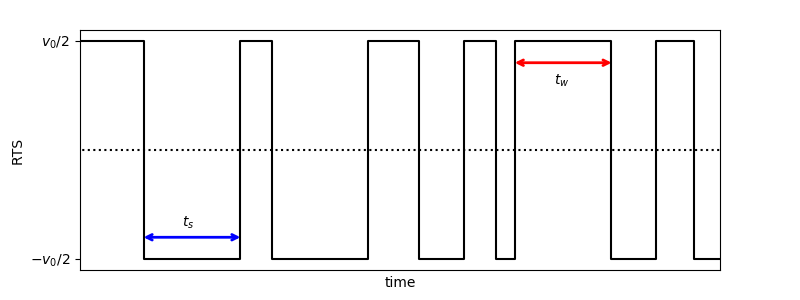
\includegraphics[width=12cm, height=5cm]{figures/2021_12_02_RTS_schematic_RTS.png}
    \caption{Schematic of a random telegraph signal with only two distinct values ($\pm v/2$) the signal can produce. The transition times $t_{s}$ and $t_{w}$ are hereby the times the system stays in either of the two states.}
    \label{fig:RTS_schematic}
\end{figure}


Previous work has shown that the noise in semiconductors can be attributed to trapping and releasing events of electrical charge carriers, which in turn cause random telegraph signals.  \cite{Guerrero2010} \cite{Leyris2006} \cite{Xiong2007} \cite{Machlup1954}
The power spectrum of the random switching between the logical ``0'' and ``1'' of these processes in general follows a decrease of $1/\omega^{2}$ \cite{Milstein2009} \cite{Puglisi2016}, but depends on the nature of the transition times, i.e. whether their mean is constant or not \cite{Machlup1954}.
In our instance the same is the case: the transition between two values, $v = 0$ and $v = v_{bee}$, is governed by two independent and stationary Poisson processes $P(m, \tau)$ with average transition timescales $t_{s}$ for when the bee is switching from walking to sitting and $t_{w}$ for when it changes from sitting to walking. 

\section{The Mean Squared Displacement}
\label{sec:MSD}

To determine the diffusion coefficient $D$ in equation \ref{eq:Langevin_reduce} a common method that can be used to analyse a particles trajectory is the mean squared displacement ($MSD$), which is a measure for the particles deviation from an initial reference position.
The $MSD$ is characterized as an average ensemble for the trajectories $\vec{X}_n$ of numerous particles $N$ after a time period $\tau$.

\begin{equation}
\label{eq:MSD_sum}
    MSD(\tau)\equiv\langle x^2(\tau)\rangle:=\lim\limits_{N\rightarrow\infty}\frac{1}{N}\cdot\sum\limits_{n=1}^N\left(\vec{X}_n(\tau)-\vec{X}_n(0)\right)^2  
\end{equation}

The value for $\tau$ in equation \ref{eq:MSD_sum} is equivalent to the duration of the experiments described in chapter \ref{chap:experiments} and we expect behaviour that is on average directly proportional to a power law $\tau^{\alpha}$. If $\alpha = 1$ we have a linear relationship between the MSD and $\tau$ that classifies the observed trajectories as normal diffusive, which indicates \cite{Lindner2008} little to no noise acting on the movement. For the cases with stronger noise, the $MSD$ implies saturating and sub-diffusive behaviour with $\alpha < 1$ and linearly growing and super-diffusive behaviour with $\alpha > 1$.

\begin{figure}
    \centering
    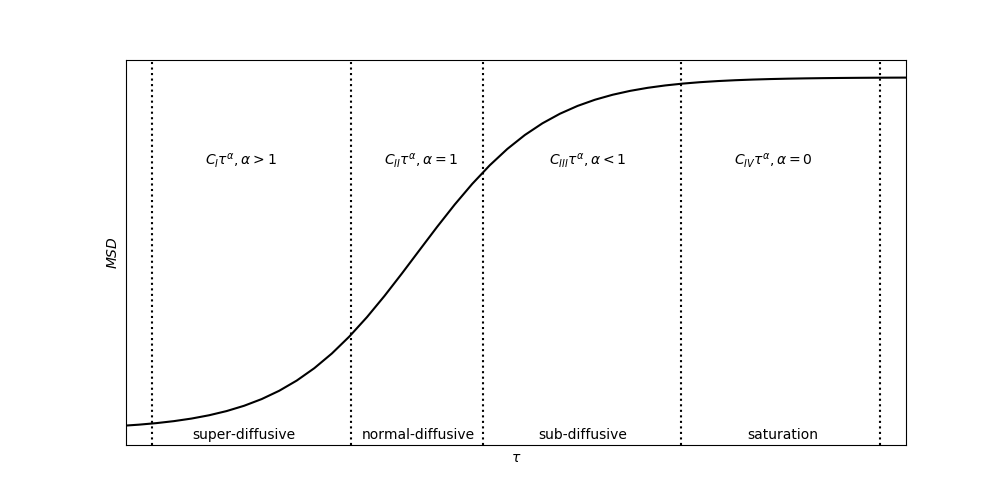
\includegraphics[width=14cm, height=7cm]{figures/2021_12_02_RTS_schematic_MSD.png}
    \caption{Schematic of a mean squared displacement over a given time domain. The progression shows a power law $\tau^{\alpha}$ first with $\alpha > 1$, continuing with a linear increase where $\alpha \approx 1$ and a saturating section where $\alpha \ll 1$, which ends in a plateau and $\alpha=0$. The different types of functions of these zones describe different grades of diffusivity.}
    \label{fig:MSD_schematic}
\end{figure}

If a statement needs to be made about the individual experimental runs, hence individual particles $N$, the $MSD$ can be redefined through a time average of a single trajectory $\vec{X}(t)$ as

\begin{equation}
\label{eq:MSD_int}
    TMSD(\tau) \equiv \langle x^2(\tilde{t})\rangle:=\lim\limits_{\tilde{T}\rightarrow\infty}\frac{1}{\tilde{T}}\cdot\int\limits_0^{\tilde{T}}\left(\vec{X}(t+\tilde{t})-\vec{X}(t)\right)^2\;\mathrm{d}t
\end{equation}

which delivers a measure for how much a particle has been displaced between times $t$ and $t+\tilde{t}$ for all possible $\tilde{t}$ within the duration $\tilde{T}$.

Another possibility to look at the data has a different and rather numerical approach, introducing the concept of a boundary to the system, where the coordinates of every collision with the arenas walls are treated as a new starting point $t_{0}$ for the $MSD$ and then averaged over the whole family of resulting curves $M$.

\begin{equation}
\label{eq:MSD_coll}
    SMSD(\tau) \equiv \langle x^{2}_M(t) \rangle := \frac{1}{M}\cdot\sum\limits_{m=1}^M|\vec{x}_m(t) - \vec{x}_m(t_{0})|^{2}
\end{equation}

The expectation that the results will indicate a behaviour ranging from sub- to super-diffusive holds true for equations \ref{eq:MSD_int} and \ref{eq:MSD_coll} as well.

\section{$1 / \omega^{2}$ Noise and the Power Spectral Density}
\label{sec:PSD}

%In time series analysis it is useful to look for recurring patterns in the data points and the power spectrum or power spectral density (PSD) is on that account an practical way to find the frequency components the data consists of.
%[TODO sentence]The Wiener-Khinchin theorem [TODO Cite Wiener 1930, Khinchin 1934] states that the autocorrelation function of a stationary random process has a spectral configuration that is given by the power spectrum of that process.
%But useful information can be extracted even if the signal is indicating that white noise is the dominating influence by analysing the power spectrum behaviour over a range of 
In time series analysis it is common to investigate a non-periodic signal in regard of its noise ratio. To do that, one can look at its spectral content via the power spectral density (PSD). It is represented as the power per unit of bandwidth of the frequency domain of a given time series. Thereby different slopes of the PSD indicate different processes and types of noise, describing in this instance different types of bee behaviour. 
White or thermal noise is characterised by a flat spectral density, meaning that it shows that same intensity, or amplitude over the whole range of the frequency domain. Brownian noise, or noise that drops proportional to $1/\omega_{2}$ can be an indicator for Brownian motion, and $1/\omega$ can have a multitude of different reasons \cite{Milotti1995}. It is well understood inside a context of transported electrons in electronic devices or dynamics within biophysics \cite{Dewey1992} \cite{Clay1976}, and will be further discussed in section \ref{sec:RTS}.

\begin{figure}[H]
    \centering
    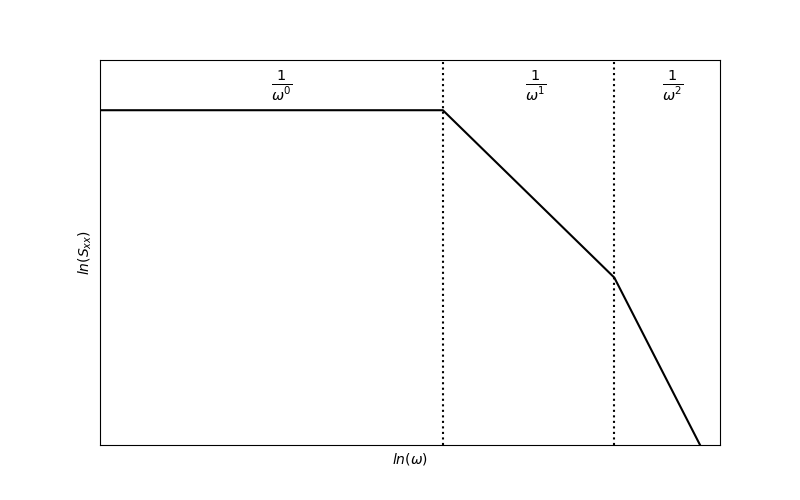
\includegraphics[width=14cm, height=8cm]{figures/2021_12_02_RTS_schematic_PSD.png}
    \captionsetup{width=12cm}
    \caption{Schematic of a power spectral density with an amplitude of a frequency range. Usually displayed in double logarithmic plots. The rate of change of the amplitude are an indicator for different kinds of noise that act on a system. The amplitude thereby follows a decrease proportional to $1/\omega^{\alpha}$ with different exponents $\alpha$, which stand for different types of noise. A system that can be described by Gaussian white noise has a power spectrum that is constant. Systems with a $1/\omega$ or $1/\omega^{2}$ decrease of the PSD are common to pink noise and brown noise respectively.}
    \label{fig:PSD_schematic}
\end{figure}

The Wiener-Khinchin theorem states, that the PSD can in general be defined as the Fourier transform of the auto-correlation function of any signal $x(t)$ \cite{Wiener1930} \cite{Khintchine1934}

\begin{equation}
\label{eq:PSD_base}
    PSD \equiv S_{xx}(\omega) := \tilde{X}^{\dagger}(\omega) \cdot \tilde{X}(\omega) = |\tilde{X}(\omega)|^{2}
\end{equation}

with

\begin{equation}
\label{eq:FT}
    \tilde{X}(\omega) = \int{x(t) \cdot e^{-\imath \omega t}}dt
\end{equation}

\subsection{Power Spectral Density of $\theta(t)$}

The power spectra for the angle $\theta$ are expected to be dependent on the temperature gradient, assuming that it acts as if a little spring is attached to the bees direction, pulling it to the higher temperature and more easily into the optimum. A PSD that scales with $1/\omega^{2}$ would indicate simple Brownian motion and no dependence on the temperature, and a progression, that flattens into a $1/\omega$ scaling or saturates entirely at some point, illustrates a dependence. Noteworthy at this point is the fact, that a well potential (or a literal wall) could lead to a flattening of the PSD as well

Inserting the Langevin equation for the angle $\theta$ (Eq.:\ref{eq:Langevin_theta}) into equation \ref{eq:FT} will result in the Fourier transform 

\begin{equation}
\label{eq:Langevin_FT}
    \imath\omega\tilde{\theta}(\omega)=-a_{\theta}\left(\tilde{\theta}(\omega)-\theta_{0}\delta(\omega)\right)+\sqrt{2D_{\theta}}\tilde{\eta}(\omega)
\end{equation}

The term containing $\theta_{0}$ can be neglected by subtracting the average angle $\theta$ from the time series before Fourier transforming it, and finally after solving for $\tilde{\theta}(\omega)$ we get

\begin{equation}
\label{eq:theta_FT}
    \tilde{\theta}(\omega) = \frac{\sqrt{2\ D_{\theta}}\tilde{\eta}(\omega)}{\imath\omega+a_{\theta}}
\end{equation}

The power spectral density on a time domain $T$ is given by

\begin{equation}
\label{eq:PSD_theta}
    S_{\theta} = \frac{1}{T}\langle|\tilde{\theta}(\omega)|^{2}\rangle =\frac{1}{T}\langle\tilde{\theta^{\dagger}}(\omega)\tilde{\theta}(\omega)\rangle
\end{equation}

Inserting $\tilde{\theta}(\omega)$ from \ref{eq:theta_FT} into \ref{eq:PSD_theta} results in

\begin{equation}
    S_{\theta} = \frac{2\ D_{\theta}\langle\tilde{\eta}^{\dagger}(\omega)\tilde{\eta}(\omega)\rangle\frac{1}{T}}{(\imath\omega+a_{\theta})(-\imath\omega+a_{\theta})}
\end{equation}

with the noise term $\langle\tilde{\eta}^{\dagger}(\omega)\tilde{\eta}(\omega)\rangle\frac{1}{T}$ being equal to $1$ (see equation \ref{eq:noise_theta}. This results in a power spectrum that gets its shape over the frequency domain $\omega$ through the two values of $D_{\theta}$ and $a_{\theta}$ and scaling with $1/\omega^{2}$.

\begin{equation}
    S_{\theta} = \frac{2D_{\theta}}{\omega^{2}+a_{\theta}^{2}}
\end{equation}

For low $\omega$ we expect a behaviour dominated by $2\ D_{\theta}/a_{\theta}^{2}$, for high $\omega$ we will see a drop off proportional to $1/\omega^{2}$. Acquiring the values for the two factors $D_{\theta}$ and $a_{\theta}$ can then be done through the comparison with the experimental data.

\subsection{Power Spectral Density of $v_{0}(t)$}

The same can be done for the velocity analogously, defining its PSD as 

\begin{equation}
\label{eq:PSD_velocity}
    S_{v}(\omega) = \frac{2D_{v}}{\omega^{2}+a_{v}^{2}}
\end{equation}

\subsection{Power Spectral Density of a Random Telegraph Signal}
\label{sec:RTS}

We begin by moving the telegraph signal by a constant factor of $v_{bee}/2$ and calculating the autocovariance of the signal, considering all the even and uneven transition probabilities as

\begin{equation}
\label{eq:Corr_vivj}
    C_{v_{i,j}}(t)=\sum\limits_{i}\sum\limits_{j}v_{i}v_{j}P\Big(v(s)=v_{i}\Big)P\Big(v(s+t) = v_{j}\Big| v(s)=v_{i}\Big)
\end{equation}

and through insertion of the Poission distribution

\begin{equation}
\label{eq:Poisson}
    P(m,\tau) = \frac{(\nu \tau) ^ {m}}{m!} e^{-\nu \tau} 
\end{equation}

into \ref{eq:Corr_vivj} the autocovariance $C_{\tau}$ gets out as

\begin{equation} 
\label{eq:Covariance}
\begin{split}
C_{\tau} & = \Big(\frac{v_{0}}{2}\Big)^2 [P(0,\tau) + P(2,\tau) + \cdots ] - \Big(\frac{v_{0}}{2}\Big)^2 [P(1,\tau) + P(3,\tau) + \cdots ] \\
         & = \Big(\frac{v_{0}}{2}\Big)^2 e^{-\nu \tau} \Big[1 - \nu \tau + \frac{(\nu \tau)^2}{2} - \frac{(\nu \tau)^3}{3!} + \frac{(\nu \tau)^4}{4!} - \cdots \Big] \\
         & = \Big(\frac{v_{0}}{2}\Big)^2 e^{-2 \nu \tau}
\end{split}
\end{equation}

Inserting the result of \ref{eq:Covariance} into the Wiener-Kinchin theorem

\begin{equation}
\label{eq:Wiener_Kinchin}
    S(\tau,\omega)=2\int\limits_{0}^{\infty}C_{\tau}\cos(\omega \tau)d \tau
\end{equation}

applying two times integration by parts and defining

\begin{equation}
    2 \nu = \Big[ \frac{1}{t_{s}} +  \frac{1}{t_{w}} \Big]
\end{equation}

the power spectral density can be formulated as

\begin{equation}
\label{eq:PSD_vivj}
   \implies S_{v}(t_{s},t_{w},\omega)=\frac{2v_{bee}^{2}}{(t_{s}+t_{w})\Big(\big(\frac{1}{t_{s}}+\frac{1}{t_{w}}\big)^{2}+\omega^{2}\Big)}
\end{equation}

For a set of times $t_{w}$, $t_{s}$ that are constant, equation \ref{eq:PSD_vivj} leads to a Lorentzian shape of the power spectrum.
We can now assume that $t_{s}$ is a variable dependent on the local temperature and is following a distribution of some kind, as a sitting bee constantly reassesses if the current position is a convenient one. At the same time we expect $t_{w}$ to be less temperature dependent, if it shows any dependence at all, as the sole act of walking suggests, that whatever the local temperature is, it is not accepted as an adequate spot.
\\
Therefore defining the difference between the local and the optimal temperature as

\begin{equation}
    \Delta T = \big|T_{local} - T_{optimum}\big|
\end{equation}

allows us to add the temperature dependence, integrate over the whole span of $\Delta T$ and rewrite \ref{eq:PSD_vivj} as

\begin{equation}
\label{eq:PSD_RTS}
    S_{RT} \coloneqq S_{v}(\omega)=2v_{bee}^{2}\int\limits_{0}^{\Delta T_{max}}\frac{P(\Delta T)d\Delta T}{\big(t_{s}(\Delta T)+t_{w}\big)\Big(\big(\frac{1}{t_{s}(\Delta T)}+\frac{1}{t_{w}}\big)^{2}+\omega^{2}\Big)}
\end{equation}

with $P(\Delta T)$ being the probability of being at a temperature $T$ and $\Delta T_{max}$ being the maximum deviation from the optimum temperature.

We now acquired two custom models for the velocity $v(t)$ and two descriptions of the respective power spectral densities (equation \ref{eq:PSD_velocity} and \ref{eq:PSD_RTS}), which we will compare to the experimental results. 

%\section{Computational Methods/Numerical Procedures}
%To calculate the needed values from the dataset and to fit the equations to them was done numerically by using the programming language "Python 3.6".
%The code can be found in the appendix chapter \ref{cha:Appendix}.
%\subsubsection{Calculation of $S_{\theta}$}
%The numerical procedure to calculate $S_{\theta}$ from the data arrays is to first calculate the Fourier transform using the "Fast Fourier Transformation" algorithm (FFT) on the "Discrete Fourier Transformation" (DFT) function of the angle $\theta(t)$:
%\begin{equation}
%\label{eq:DFT}
%    \tilde{\theta}_{k}=\sum\limits^{N-1}_{n=0}\theta_{n}[\cos\frac{2\pi}{N}kn-\imath\sin\frac{2\pi}{N}kn]
%\end{equation}
%where $T=N dt$ and $\omega=2\pi k$. \\
%As the FFT returns a vector in the complex plane $\mathbb{C}$, the spectral density then can be acquired through
%\begin{equation}
%    S_{\theta}(\omega) = \frac{1}{T}\left(\mathbf{Re}[\tilde{\theta}(\omega)]^2 + \mathbf{Im}[\tilde{\theta}(\omega)]^2\right)
%\end{equation}
%\subsubsection{Fast Fourier Transformation}
%\subsubsection{Fitting methods}
%\subsubsection{Box Muller Transformation}
%[table of used libraries ]